
\de{ĐỀ THI HỌC KỲ I NĂM HỌC 2022-2023}{THPT Chuyên Quốc Học Huế - Huế}
\begin{center}
	\textbf{PHẦN 1 - TRẮC NGHIỆM}
\end{center}
\Opensolutionfile{ans}[ans/ans]
%Câu1
\begin{ex}%[0D1Y2-1]%[Dự án đề kiểm tra HKI NH22-23- Phan Trung Hiếu]%[THPT Chuyên Quốc học - Huế]
	Tập hợp $A=\{x\in\mathbb{N}|-3\leq x\leq 3\}$ có bao nhiêu phần tử?
	\choice
	{$5$}
	{\True $4$}
	{$7$}
	{$6$}
	\loigiai{
		Ta có $A=\{0;1;2;3\}$. Do đó tập hợp $A$ có 4 phần tử.
	}
\end{ex}
%Câu2
\begin{ex}%[0H2Y1-2]%[Dự án đề kiểm tra HKI NH22-23- Phan Trung Hiếu]%[THPT Chuyên Quốc học - Huế]
	Cho véc-tơ $\vec{a}$ tùy ý, khác $\vec{0}$ và $k$ là số thực bất kì. Phát biểu nào sau đây là \textbf{sai}?
	\choice
	{$|k\vec{a}|=|k||\vec{a}|$}
	{$\vec{a}$ và $-\vec{a}$ là hai véc-tơ ngược huớng}
	{Nếu $\vec{a}$ và $k\vec{a}$ cùng huớng thì $k>0$}
	{\True $\vec{a}$ và $k\vec{a}$ là hai véc-tơ cùng phương với mọi $k$}
	\loigiai{
		$\vec{a}$ và $k\vec{a}$ là hai véc-tơ cùng phương với mọi $k\ne 0$.
	}
\end{ex}
%Câu3
\begin{ex}%[0H2Y4-1]%[Dự án đề kiểm tra HKI NH22-23- Phan Trung Hiếu]%[THPT Chuyên Quốc học - Huế]
	Cho hai véc-tơ tùy ý $\vec{a}$ và $\vec{b}$ đều khác $\vec{0}$. Mệnh đề nào dưới đây \textbf{đúng}?
	\choice
	{\True $\vec{a}\cdot\vec{b}=|\vec{a}|\cdot|\vec{b}|\cdot\cos(\vec{a},\vec{b})$}
	{$\vec{a}\cdot\vec{b}=-|\vec{a}|\cdot|\vec{b}|$}
	{$\vec{a}\cdot\vec{b}=|\vec{a}|\cdot|\vec{b}|$}
	{$\vec{a}\cdot\vec{b}=|\vec{a}|\cdot|\vec{b}|\cdot\sin(\vec{a},\vec{b})$}
	\loigiai{
		Công thức tích vô huớng của hai véc-tơ là $\vec{a}\cdot\vec{b}=|\vec{a}|\cdot|\vec{b}|\cdot\cos(\vec{a},\vec{b})$.
	}
\end{ex}
%Câu4
\begin{ex}%[0X1B4-3]%[Dự án đề kiểm tra HKI NH22-23- Phan Trung Hiếu]%[THPT Chuyên Quốc học - Huế]
	Điểm trung bình từng môn học kì I môn Toán của bạn An được cho bởi bảng sau
	\begin{center}
		\begin{tabular}{|c|c|c|c|c|c|c|c|c|}
			\hline
			Môn&Toán&Vật Lí&Hóa học&Ngữ văn&Lịch sử&Địa lí&Tin học&Tiếng anh\\
			\hline
			Điểm&$9{,}1$&$8{,}6$&$9{,}3$&$6{,}8$&$8{,}0$&$7{,}5$&$8{,}7$&$6{,}8$\\
			\hline
		\end{tabular}
	\end{center}
	Phương sai của mẫu số liệu trên bằng
	\choice
	{$0{,}92$}
	{$2{,}5$}
	{\True $0{,}85$}
	{$0{,}72$}
	\loigiai{
		Điểm trung bình của tất cả các môn học là
		\begin{equation*}
			\overline{x}=\dfrac{9{,}1 + 8{,}6 + 9{,}3 + 6{,}8 + 8{,}0 + 7{,}5 + 8{,}7 + 6{,}8}{8} = 8{,}1.
		\end{equation*}
		Phương sai của mâu số liệu trên là
		\begin{eqnarray*}
			 &\dfrac{1}{8}[(9{,}1 - 8{,}1)^2&+ (8{,}6 - 8{,}1)^2 + (9{,}3 - 8{,}1)^2 + (6{,}8 - 8{,}1)^2 \\
			&+(8{,}0 - 8{,}1)^2& + (7{,}5 - 8{,}1)^2 + (8{,}7 - 8{,}1)^2 + (6{,}8 - 8{,}1)^2 ]\approx 0{,}85.
		\end{eqnarray*}
	}
\end{ex}
%Câu5
\begin{ex}%[0H2B1-1]%[Dự án đề kiểm tra HKI NH22-23- Phan Trung Hiếu]%[THPT Chuyên Quốc học - Huế]
	Từ 3 điểm phân biệt $A$, $B$, $C$ có thể lập được bao nhiêu véc-tơ khác $\vec{0}$ có điểm đầu và điểm cuối là các điểm đã cho?
	\choice
	{\True $6$}
	{$9$}
	{$4$}
	{$3$}
	\loigiai{
		Số véc-tơ khác $\vec{0}$ có điểm đầu và điểm cuối là các điểm đã cho là $A_3^2=6$.
	}
\end{ex}
%Câu6
\begin{ex}%[0D1Y1-3]%[Dự án đề kiểm tra HKI NH22-23- Phan Trung Hiếu]%[THPT Chuyên Quốc học - Huế]
	Cho mệnh đề $P\colon\lq\lq\exists x\in\mathbb{R},x^2-1=0\lq\lq$. Mệnh đề nào sau đây là mệnh đề phủ định của mệnh đề $P$?
	\choice
	{$\overline{P}\colon\lq\lq\exists x\in\mathbb{R},x^2-1\ne0\lq\lq$}
	{$\overline{P}\colon\lq\lq\forall x\in\mathbb{R},x^2-1=0\lq\lq$}
	{\True $\overline{P}\colon\lq\lq\forall x\in\mathbb{R},x^2-1\ne0\lq\lq$}
	{$\overline{P}\colon\lq\lq\forall x\in\mathbb{R},x^2-1>0\lq\lq$}
	\loigiai{
		Mệnh đề phủ định của mệnh đề $P$ là $\overline{P}\colon\lq\lq\forall x\in\mathbb{R},x^2-1\ne0\lq\lq$.
	}
\end{ex}
%Câu7
\begin{ex}%[0H1Y2-1]%[Dự án đề kiểm tra HKI NH22-23- Phan Trung Hiếu]%[THPT Chuyên Quốc học - Huế]
	Cho tam giác $ABC$ với các cạnh $AB=c$, $AC=b$, $BC=a$. Gọi $R$, $r$, $S$ lần lượt là bán kính đường tròn ngoại tiếp, bán kính đường tròn nội tiếp, diện tích của tam giác $ABC$. Trong các khẳng định sau đây, khẳng định nào là \textbf{sai}?
	\choice
	{$S=\dfrac{abc}{4R}$}
	{$S=\dfrac{1}{2}ab\sin C$}
	{\True $R=\dfrac{b}{\sin B}$}
	{$c^2=a^2+b^2-2ab\cdot\cos C$}
	\loigiai{
		Theo định lý sin $2R=\dfrac{b}{\sin B}$.
	}
\end{ex}
%Câu8
\begin{ex}%[0X1Y3-2]%[Dự án đề kiểm tra HKI NH22-23- Phan Trung Hiếu]%[THPT Chuyên Quốc học - Huế]
	Thu thập hàng tháng (đơn vị: triệu đồng) của 7 nhân viên trong một công ty A được cho như sau $$3{,}5\quad6{,}5\quad6{,}8\quad7{,}2\quad8{,}2\quad8{,}5\quad9{,}2$$ Số trung vị của mẫu số liệu trên bằng
	\choice
	{$6{,}8$}
	{$3{,}5$}
	{$9{,}2$}
	{\True $7{,}2$}
	\loigiai{
		Mẫu số liệu gồm 7 số liệu nên số trung vị của mẫu số liệu là $M_e=7{,}2$
	}
\end{ex}
%Câu9
\begin{ex}%[0H2B4-1]%[Dự án đề kiểm tra HKI NH22-23- Phan Trung Hiếu]%[THPT Chuyên Quốc học - Huế]
	Cho tam giác $ABC$ vuông tại $A$ có $\widehat{B}=40^\circ$. Hệ thức nào sau đây là \textbf{sai}?
	\choice
	{\True $(\vv{AC},\vv{CB})=50^\circ$}
	{$(\vv{BC},\vv{AC})=50^\circ$}
	{$(\vv{AB},\vv{CB})=40^\circ$}
	{$(\vv{AB},\vv{BC})=140^\circ$}
	\loigiai{
		Vẽ véc-tơ $\vv{AD}$ sao cho $\vv{AD}=\vv{CB}$.
		\begin{center}
			\begin{tikzpicture}[font=\footnotesize, thick]
				\path 
				(0,0) coordinate (A)
				(90:3) coordinate (C)
				(5,0) coordinate (B)
				($(A)+(B)-(C)$) coordinate (D)
				;
				\draw (A)--(C)--(B)--(D)--cycle (A)--(B);
				\draw pic["$40^\circ$",-stealth,angle radius=15mm]{angle=C--B--A};
				\draw pic[draw,angle radius=2mm]{right angle=C--A--B};%Theo chiều dương
				\foreach \x/\g in {A/-90,B/0,C/90,D/0}
				\fill[black] 	(\x) circle (1pt)
				($(\g:3mm)+(\x)$) node {$\x$};
			\end{tikzpicture}
		\end{center}
		Vì $\vv{AD}=\vv{CB}$ nên tứ giác $ACBD$ là hình bình hành và do đó $\widehat{ABC}=\widehat{DAB}=40^\circ$.\\
		Ta có $(\vv{AC},\vv{CB})=(\vv{AC},\vv{AD})=90^\circ+40^\circ = 130^\circ$.
	}
\end{ex}
%Câu10
\begin{ex}%[0H2B3-4]%[Dự án đề kiểm tra HKI NH22-23- Phan Trung Hiếu]%[THPT Chuyên Quốc học - Huế]
	Trong mặt phẳng tọa độ $Oxy$, cho $A(1;1)$, $B(-2;7)$, $C(0;m)$. Tìm $m$ để $A$, $B$, $C$ thẳng hàng.
	\choice
	{$m=1$}
	{$m=-9$}
	{$m=-1$}
	{\True $m=3$}
	\loigiai{
		Ta có $\vv{AB}=(-3,6)$ và $\vv{AC}=(-1,m-1)$. $A$, $B$, $C$ thẳng hàng khi và chỉ khi
		\begin{equation*}
			\dfrac{-1}{-3}=\dfrac{m-1}{6}\Leftrightarrow m =3.
		\end{equation*}
	}
\end{ex}
%Câu11
\begin{ex}%[0H2B3-2]%[Dự án đề kiểm tra HKI NH22-23- Phan Trung Hiếu]%[THPT Chuyên Quốc học - Huế]
	Trong mặt phẳng tọa độ $Oxy$ với véc-tơ đơn vị $\vec{i}$ của trục $Ox$ và véc-tơ đơn vị $\vec{j}$ của trục $Oy$, cho $\vec{u}+2\vec{i}-3\vec{j}=\vec{0}$. Tìm tọa độ của véc-tơ $\vec{u}$.
	\choice
	{$\vec{u}=(3;-2)$}
	{$\vec{u}=(2;-3)$}
	{$\vec{u}=(-3;2)$}
	{\True $\vec{u}=(-2;3)$}
	\loigiai{
		Ta có $\vec{u} = 3\vec{j}-2\vec{i} = 3\cdot(0;1)-2\cdot(1;0) = (-2;3)$.
	}
\end{ex}
%Câu12
\begin{ex}%[0H2B3-6]%[Dự án đề kiểm tra HKI NH22-23- Phan Trung Hiếu]%[THPT Chuyên Quốc học - Huế]
	Cho tam giác $ABC$ đều, độ dài cạnh bằng 1. Tính $|\vv{AB}+\vv{AC}|$.
	\choice
	{$\dfrac{\sqrt{3}}{2}$}
	{\True $\sqrt{3}$}
	{$\sqrt{2}$}
	{$1$}
	\loigiai{
		Gọi $M$ là trung điểm của cạnh $BC$, khi đó $|\vv{AB}+\vv{AC}| = |2\vv{AM}| = 2AM = \sqrt{3}$.
	}
\end{ex}
%Câu13
\begin{ex}%[0D2Y1-2]%[Dự án đề kiểm tra HKI NH22-23- Phan Trung Hiếu]%[THPT Chuyên Quốc học - Huế]
	Miền nghiệm của bất phương trình $x+2(y-1)>x+4$ chứa điểm nào sau đây?
	\choice
	{$Q(6;0)$}
	{\True $P(-5;5)$}
	{$M(-2;1)$}
	{$N(1;3)$}
	\loigiai{
		Thay $P(-5;5)$ vào $x+2(y-1)>x+4$ ta được $3>-1$ (đúng), do đó miền nghiệm của bất phương trình $x+2(y-1)>x+4$ chứa điểm $P$.
	}
\end{ex}
%Câu14
\begin{ex}%[0H2B4-4]%[Dự án đề kiểm tra HKI NH22-23- Phan Trung Hiếu]%[THPT Chuyên Quốc học - Huế]
	Trong mặt phẳng tọa độ $Oxy$, cho hai véc-tơ $\vec{a}=(2m-1;-3)$ và $\vec{b}=(1;-3)$. Tìm $m$ để $\vec{a}\perp\vec{b}$.
	\choice
	{$m=3$}
	{$m=1$}
	{\True $m=-4$}
	{$m=5$}
	\loigiai{
		$\vec{a}\perp\vec{b}$ khi và chỉ khi $(2m-1)\cdot1+9 = 0\Leftrightarrow m =-4$.
	}
\end{ex}
%Câu15
\begin{ex}%[0X1Y4-1]%[Dự án đề kiểm tra HKI NH22-23- Phan Trung Hiếu]%[THPT Chuyên Quốc học - Huế]
	Điểm kiểm tra học kì I môn Toán của 8 học sinh tổ 1 lớp 10A được cho như sau
	\begin{equation*}
		8\quad6\quad7\quad8\quad9\quad10\quad9\quad7.
	\end{equation*}Khoảng biến thiên của mẫu số liệu trên là
	\choice
	{\True $R=4$}
	{$R=3$}
	{$R=2$}
	{$R=1$}
	\loigiai{
		Sắp xếp mẫu số liệu theo thứ tự không giảm
		\begin{equation*}
			6\quad7\quad7\quad8\quad8\quad9\quad9\quad10
		\end{equation*}
		Giá trị nhỏ nhất là $6$.\\
		Giá trị lớn nhất là $10$.\\
		Khoảng biến thiên của mẫu số liệu là $R = 10 - 6 = 4$.
	}
\end{ex}
%Câu16
\begin{ex}%[0H3Y2-1]%[Dự án đề kiểm tra HKI NH22-23- Phan Trung Hiếu]%[THPT Chuyên Quốc học - Huế]
	Cho tam giác đều $ABC$ cạnh $a$. Tính $\vv{CA}\cdot\vv{CB}$.
	\choice
	{$a^2$}
	{$\dfrac{a^2\sqrt{3}}{2}$}
	{\True$\dfrac{a^2}{2}$}
	{$-a^2$}
	\loigiai{
		$\vv{CA}\cdot\vv{CB} = \left|\vv{CA}\right|\cdot\left|\vv{CB}\right|\cdot\cos(\vv{CA},\vv{CB})=a\cdot a\cdot\cos 60^\circ = \dfrac{a^2}{2}$.
	}
\end{ex}
%Câu17
\begin{ex}%[0H2Y2-3]%[Dự án đề kiểm tra HKI NH22-23- Phan Trung Hiếu]%[THPT Chuyên Quốc học - Huế]
	Cho 2 véc-tơ tùy ý $\vec{a}$ và $\vec{b}$. Mệnh đề nào dưới đây \textbf{đúng}?
	\choice
	{$|\vec{a}+\vec{b}|\geq|\vec{a}|+|\vec{b}|$}
	{$|\vec{a}+\vec{b}|>|\vec{a}|+|\vec{b}|$}
	{\True $|\vec{a}+\vec{b}|\leq|\vec{a}|+|\vec{b}|$}
	{$|\vec{a}+\vec{b}|<|\vec{a}|+|\vec{b}|$}
	\loigiai{
		
	}
\end{ex}
%Câu18
\begin{ex}%[0H3K1-3]%[Dự án đề kiểm tra HKI NH22-23- Phan Trung Hiếu]%[THPT Chuyên Quốc học - Huế]
	Trong mặt phẳng tọa độ $Oxy$, cho $M(1;2)$, $N(-3;1)$, $P(0;6)$ lần lượt là trung điểm các cạnh $BC$, $CA$, $AB$ của tam giác $ABC$. Tìm tọa độ đỉnh $C$.
	\choice
	{$(-4;-7)$}
	{\True $(-2;-3)$}
	{$(4;7)$}
	{$(-4;5)$}
	\loigiai{
		Gọi $A(x_A,y_A)$, $B(x_B,y_B)$, $C(x_C,y_C)$.\\
		Vì $M$ là trung điểm của $BC$ nên ta có
		\begin{equation*}
			\heva{&1=\dfrac{x_B+x_C}{2}\\&2=\dfrac{y_B+y_C}{2}}\Leftrightarrow\heva{&x_B+x_C=2\\&y_B+y_C=4.}
		\end{equation*}
		Vì $N$ là trung điểm của $CA$ nên ta có
		\begin{equation*}
			\heva{&-3=\dfrac{x_C+x_A}{2}\\&1=\dfrac{y_C+y_A}{2}}\Leftrightarrow\heva{&x_C+x_A=-6\\&y_C+y_A=2.}
		\end{equation*}
		Vì $P$ là trung điểm của $AB$ nên ta có
		\begin{equation*}
			\heva{&0=\dfrac{x_A+x_B}{2}\\&6=\dfrac{y_A+y_B}{2}}\Leftrightarrow\heva{&x_A+x_B=0\\&y_A+y_B=12.}
		\end{equation*}
		Do đó, ta có các hệ phương trình sau
		\begin{equation*}
			\heva{&x_B+x_C=2\\&x_C+x_A=-6\\&x_A+x_B=0}\Leftrightarrow\heva{&x_A=-4\\&x_B=4\\&x_C=-2,}
		\end{equation*}
		và
		\begin{equation*}
			\heva{&y_B+y_C=4\\&y_C+y_A=2\\&y_A+y_B=12}\Leftrightarrow\heva{&y_A=5\\&y_B=7\\&y_C=-3.}
		\end{equation*}
		Vậy tọa độ điểm $C$ là $C(-2;-3)$.
	}
\end{ex}
%Câu19
\begin{ex}%[D2Y1-1]%[Dự án đề kiểm tra HKI NH22-23- Phan Trung Hiếu]%[THPT Chuyên Quốc học - Huế]
	Bất phương trình nào sau đây \textbf{không} là bất phương trình bậc nhất hai ẩn?
	\choice
	{$x\leq 2y$}
	{$x+y<0$}
	{$2022x+y\geq2023$}
	{\True $x(x-1)+y>0$}
	\loigiai{
		Bất phương trình bậc nhất hai ẩn có dạng $ax+by+c>0$.\\
		Vì $x(x-1)+y$ có bậc là hai nên bất phương trình $x(x-1)+y>0$ không là bất phương trình bậc nhất hai ẩn.
	}
\end{ex}
%Câu20
\begin{ex}%[0H2K2-3]%[Dự án đề kiểm tra HKI NH22-23- Phan Trung Hiếu]%[THPT Chuyên Quốc học - Huế]
	Cho tam giác $ABC$ có trọng tâm $G$ và $I$ là trung điểm của $BG$. Biểu diễn véc-tơ  $\vv{AI}$ qua hai véc-tơ $\vv{AB}$ và $\vv{AC}$.
	\choice
	{$\vv{AI}=\dfrac{1}{2}\vv{AB}+\dfrac{1}{4}\vv{AC}$}
	{$\vv{AI}=\dfrac{3}{4}\vv{AB}+\dfrac{1}{8}\vv{AC}$}
	{$\vv{AI}=\dfrac{4}{3}\vv{AB}+\dfrac{1}{6}\vv{AC}$}
	{\True $\vv{AI}=\dfrac{2}{3}\vv{AB}+\dfrac{1}{6}\vv{AC}$}
	\loigiai{
		\begin{center}
			\begin{tikzpicture}[font=\footnotesize, thick]
				\path 
				(0,0) coordinate (B)
				(1,3) coordinate (A)
				(5,0) coordinate (C)
				($ (A)!0.5!(B) $) coordinate (P)
				($ (B)!0.5!(C) $) coordinate (M)
				($ (A)!0.5!(C) $) coordinate (N)
				(intersection of A--M and B--N) coordinate (G)
				($ (B)!0.5!(G) $) coordinate (I)
				;
				\draw (A)--(B)--(C)--cycle (A)--(M) (B)--(N) (C)--(P) (A)--(I);
				\foreach \x/\g in {A/90,B/180,C/0,I/-90,G/60,M/-90}
				\fill[black] 	(\x) circle (1pt)
				($(\g:3mm)+(\x)$) node {$\x$};
			\end{tikzpicture}
		\end{center}
		Ta có $\vv{AI} = \dfrac{1}{2}\vv{AB}+\dfrac{1}{2}\vv{AG}$ (vì $I$ là trung điểm của $BG$).\\
		Mặt khác, do $G$ là trọng tâm của tam giác $ABC$ và gọi $M$ là trung điểm của $BC$ nên
		\begin{equation*}
			\vv{AG} = \dfrac{2}{3}\vv{AM} = \dfrac{2}{3}\left(\dfrac{1}{2}\vv{AB}+\dfrac{1}{2}\vv{AC}\right) = \dfrac{1}{3}\vv{AB}+\dfrac{1}{3}\vv{AC}.
		\end{equation*}
		Suy ra,
		\begin{equation*}
			\vv{AI}=\dfrac{1}{2}\vv{AB}+\dfrac{1}{2}\left(\dfrac{1}{3}\vv{AB}+\dfrac{1}{3}\vv{AC}\right) = \dfrac{2}{3}\vv{AB}+\dfrac{1}{6}\vv{AC}.
		\end{equation*}
	}
\end{ex}
%Câu21
\begin{ex}%[0H2B2-3]%[Dự án đề kiểm tra HKI NH22-23- Phan Trung Hiếu]%[THPT Chuyên Quốc học - Huế]
	Cho hình thang $ABCD$ có $\vv{AD}=2\vv{BC}$, $M$ là trung điểm của $AD$. Khẳng định nào sau đây là \textbf{đúng}?
	\choice
	{$\vv{CB}+\vv{CD}=\vv{CA}$}
	{\True $\vv{AC}=\vv{AB}+\vv{AM}$}
	{$\vv{BA}+\vv{BC}=\vv{AC}$}
	{$\vv{CA}+\vv{CD}=\vv{CM}$}
	\loigiai{
		\begin{center}
		\begin{tikzpicture}[font=\footnotesize, thick]
			\path 
			(0,0) coordinate (A)
			(6,0) coordinate (D)
			(1,2) coordinate (B)
			(4,2) coordinate (C)
			($(A)!.5!(D)$) coordinate (M)
			;
			\draw (A)--(B)--(C)--(D)--cycle;
			\foreach \x/\g in {A/180,D/30,C/45,B/130,M/-90}
			\fill[black] 	(\x) circle (1pt)
			($(\g:3mm)+(\x)$) node {$\x$};
		\end{tikzpicture}
		\end{center}
		Vì $M$ là trung điểm của $AD$ nên $\vv{AD}=2\vv{AM}$, mà $\vv{AD}=2\vv{BC}$, do đó $\vv{AM}=\vv{BC}$.\\
		Suy ra, tứ giác $ABCM$ là hình bình hành.\\
		Theo hệ thức hình bình hành
		\begin{equation*}
			\vv{AC}=\vv{AB}+\vv{AM}.
		\end{equation*}
	}
\end{ex}
%Câu22
\begin{ex}%[0X1Y1-3]%[Dự án đề kiểm tra HKI NH22-23- Phan Trung Hiếu]%[THPT Chuyên Quốc học - Huế]
	Cho số gần đúng $a=1263{,}5$ với độ chính xác $d=0{,}1$. Số quy tròn của số $a$ là
	\choice
	{$1262$}
	{\True $1264$}
	{$1260$}
	{$1300$}
	\loigiai{
		Số quy tròn của số $a$ với độ chính xác $d=0{,}1$ là $1264$.
	}
\end{ex}
%Câu23
\begin{ex}%[0H3Y1-3]%[Dự án đề kiểm tra HKI NH22-23- Phan Trung Hiếu]%[THPT Chuyên Quốc học - Huế]
	Trong mặt phẳng tọa độ $Oxy$, cho $A(2;1)$, $B(-3;2)$. Tìm tọa độ véc-tơ $\vv{AB}$.
	\choice
	{$\vv{AB}=(5;-1)$}
	{$\vv{AB}=(-5;-1)$}
	{$\vv{AB}=(-1;3)$}
	{\True $\vv{AB}=(-5;1)$}
	\loigiai{
		Tọa độ véc-tơ $\vv{AB}$ là $\vv{AB}=(-3-2;2-1)=(-5;1)$.
	}
\end{ex}
%Câu24
\begin{ex}%[0H2Y3-4]%[Dự án đề kiểm tra HKI NH22-23- Phan Trung Hiếu]%[THPT Chuyên Quốc học - Huế]
	Cho $3$ điểm phân biệt $A$, $B$, $C$. Điều kiện cần và đủ để $B$ nằm giữa 2 điểm $A$ và $C$ là gì?
	\choice
	{\True $\vv{BA}$, $\vv{BC}$ cùng phương}
	{$\vv{AB}$, $\vv{AC}$ cùng phương}
	{$\vv{AB}$, $\vv{BC}$ cùng hướng}
	{$\vv{AB}$, $\vv{AC}$ cùng hướng}
	\loigiai{
		Điều kiện cần và đủ để $B$ nằm giữa 2 điểm $A$ và $C$ là $\vv{BA}$, $\vv{BC}$ cùng phương.
	}
\end{ex}
%Câu25
\begin{ex}%[0D2B2-2]%[Dự án đề kiểm tra HKI NH22-23- Phan Trung Hiếu]%[THPT Chuyên Quốc học - Huế]
	Cho hệ bất phương trình $\heva{&-x+3y\geq0\\&x-y\geq1}$ có tập nghiệm $S$. Khẳng định nào sau đây là \textbf{đúng}?
	\choice
	{\True$(1;-1)\notin S$}
	{$(-1;1)\in S$}
	{\True $(0;0)\in S$}
	{$(2;1)\in S$}
	\loigiai{
		\begin{center}
			\begin{tikzpicture}[font=\footnotesize, thick, line cap=round, line join=round, >=stealth]
				\def\xmin{-3}
				\def\xmax{3}
				\def\ymin{-3}
				\def\ymax{3}
				\clip (\xmin,\ymin) rectangle (\xmax,\ymax);
				\draw[-stealth] (\xmin,0)--(0,0)node[below left]{$O$}--(\xmax,0)node[above]{$x$};
				\draw[-stealth] (0,\ymin)--(0,\ymax)node[left]{$y$};
				\draw[domain=\xmin:\xmax,samples=200,smooth]plot (\x,{(1/3)*(\x)}) ;
				\draw[domain=\xmin:\xmax,samples=200,smooth]plot (\x,{(\x)-1}) ;
				\draw[dashed] (1,0)node[below right]{$1$}--(1,-1)node[below]{$A(1,-1)$}--(0,-1)node[above left]{$-1$};
				\draw[dashed] (-1,0)node[above left]{$-1$}--(-1,1)node[above]{$B(-1,1)$}--(0,1)node[above right]{$1$};
				\draw[dashed] (2,0)node[below]{$2$}--(2,1)node[above]{$D(2,1)$}--(0,1);
				\fill[pattern=north west lines, pattern color=pink,opacity=.7] (\xmin,\ymin)--plot[domain=\xmin:\xmax](\x,{(1/3)*(\x)})--(\xmax,\ymin);
				\fill[pattern=north east lines, pattern color=blue,opacity=.5] (\xmin,\ymax)--plot[domain=\xmin:\xmax](\x,{(\x)-1})--(\xmax,\ymax);
			\end{tikzpicture}
		\end{center}
		Miền nghiệm của hệ bất phương trình là miền không bị bao gồm cả hai đường thẳng.
	}
\end{ex}
%Câu26
\begin{ex}%[0H2B2-3]%[Dự án đề kiểm tra HKI NH22-23- Phan Trung Hiếu]%[THPT Chuyên Quốc học - Huế]
	Cho hình bình hành $ABCD$. Khẳng định nào sau đây là \textbf{sai}?
	\choice
	{$\vv{BC}$ cùng phương với $\vv{AD}$}
	{$\vv{AB}=\vv{DC}$}
	{\True $\vv{AC}=\vv{BD}$}
	{$\vv{BD}=\vv{BA}+\vv{BC}$}
	\loigiai{
		\begin{center}
		\begin{tikzpicture}[font=\footnotesize,thick]
			\path 
			(0,0) coordinate (A)
			(4,0) coordinate (B)
			(1,2) coordinate (D)
			($(D)+(B)-(A)$) coordinate (C)
			;
			\draw (A)--(B)--(C)--(D)--cycle;
			\foreach \x/\g in {A/180,B/0,C/30,D/180}
			\fill[black] 	(\x) circle (1pt)
			($(\g:3mm)+(\x)$) node {$\x$};
		\end{tikzpicture}
	\end{center}
	Dễ thấy, $\vv{BC}$ cùng phương với $\vv{AD}$ và $\vv{AB}=\vv{DC}$.\\
	Theo hệ thức hình bình hành, $\vv{BD}=\vv{BA}+\vv{BC}$.\\
	Vậy đáp án sai là C.
	}
\end{ex}
%Câu27
\begin{ex}%[0D1Y1-2]%[Dự án đề kiểm tra HKI NH22-23- Phan Trung Hiếu]%[THPT Chuyên Quốc học - Huế]
	Trong các mệnh đề sau, mệnh đề nào \textbf{đúng}?
	\choice
	{\True $\dfrac{2}{3}$ là một số hữu tỷ}
	{$19$ chia hết cho $3$}
	{$2022$ là một số lẻ}
	{$\sqrt{7}$ không phải là một số vô tỷ}
	\loigiai{
		\begin{itemize}
			\item $19$ không chia hết cho $3$.
			\item $2022$ là một số chẵn.
			\item $\sqrt{7}$ là một số vô tỷ.
		\end{itemize}
	}
\end{ex}
%Câu28
\begin{ex}%[0X1Y3-4]%[Dự án đề kiểm tra HKI NH22-23- Phan Trung Hiếu]%[THPT Chuyên Quốc học - Huế]
	Một cửa hàng bán quần áo thống kê số áo sơ mi nam đã bán ra trong một quý theo các cỡ khác nhau và có được bảng sau
	\begin{center}
		\begin{tabular}{|c|c|c|c|c|c|c|c|}
			\hline
			Cỡ áo&$36$&$37$&$38$&$39$&$40$&$41$&$42$\\
			\hline
			Số áo bán được&$12$&$46$&$120$&$174$&$116$&$50$&$5$\\
			\hline
		\end{tabular}
	\end{center}
	Giá trị mốt của mẫu số liệu trên là
	\choice
	{$174$}
	{\True $39$}
	{$5$}
	{$42$}
	\loigiai{
		Vì số áo cỡ $39$ bán được nhiều nhất là $174$ áo nên giá trị mốt của mẫu số liệu trên là $39$.
	}
\end{ex}
%Câu29
\begin{ex}%[0H2K2-6]%[Dự án đề kiểm tra HKI NH22-23- Phan Trung Hiếu]%[THPT Chuyên Quốc học - Huế]
	Một con thuyền di chuyển trên sông với vận tốc riêng được biểu diễn bởi véc-tơ $\vv{v_r}$, vận tốc của dòng nước được biểu diễn với véc-tơ $\vv{v_n}$ và vận tốc thực tế của con thuyền được biểu diễn bởi véc-tơ $\vv{v}$. Khẳng định nào sau đây là \textbf{đúng}?
	\choice
	{$|\vv{v_n}|+|\vv{v_r}|=|\vv{v}|$}
	{$\vv{v_n}-\vv{v_r}=\vv{v}$}
	{\True $\vv{v_n}+\vv{v_r}=\vv{v}$}
	{$\vv{v_r}-\vv{v_n}=\vv{v}$}
	\loigiai{
		Véc-tơ vận tốc thực tế của con thuyền $\vv{v}$ là tổng hợp của véc-tơ vận tốc của con thuyền trong điều kiện không có dòng nước $\vv{v_r}$ và véc-tơ vận tốc do dòng nước tạo ra $\vv{v_n}$.\\
		Vậy, khẳng định đúng là: $\vv{v_n} + \vv{v_r} = \vv{v}$.
	}
\end{ex}
%Câu30
\begin{ex}%[0H1Y1-2]%[Dự án đề kiểm tra HKI NH22-23- Phan Trung Hiếu]%[THPT Chuyên Quốc học - Huế]
	Trong các khẳng định sau đây, khẳng định nào là \textbf{đúng}?
	\choice
	{\True $\sin120^\circ>0$}
	{$\cos120^\circ>0$}
	{$\cot120^\circ>0$}
	{$\tan120^\circ>0$}
	\loigiai{
		Ta có $\sin120^\circ = \dfrac{\sqrt{3}}{2}>0$.
	}
\end{ex}
%Câu31
\begin{ex}%[0H2K1-5]%[Dự án đề kiểm tra HKI NH22-23- Phan Trung Hiếu]%[THPT Chuyên Quốc học - Huế]
	Cho tam giác $ABC$ đều, cạnh $a$. Gọi $M$ là điểm thỏa mãn $2\vv{MA}+\vv{MB}+\vv{MC}=\vv{0}$. Tính $|\vv{AM}|$.
	\choice
	{$\dfrac{a}{2}$}
	{$\dfrac{a\sqrt{3}}{2}$}
	{$\dfrac{a\sqrt{2}}{2}$}
	{\True $\dfrac{a\sqrt{3}}{4}$}
	\loigiai{
		Gọi $H$ là trung điểm của $BC$. Khi đó, theo hệ thức hình bình hành
		\begin{equation*}
			|\vv{AB}+\vv{AC}| = 2|\vv{AH}| = a\sqrt{3}.
		\end{equation*}
		Ta có
		\allowdisplaybreaks
		\begin{eqnarray*}
			2\vv{MA}+\vv{MB}+\vv{MC}&=&\vv{0}\Leftrightarrow4\vv{MA} + \vv{AB}+\vv{AC}=\vv{0}\\
			&\Rightarrow&4|\vv{MA}| = a\sqrt{3}\\
			&\Rightarrow&|\vv{MA}|=\dfrac{a\sqrt{3}}{4}\\
			&\Leftrightarrow&|\vv{AM}|=\dfrac{a\sqrt{3}}{4}.
		\end{eqnarray*}
		Vậy $|\vv{AM}|=\dfrac{a\sqrt{3}}{4}$.
	}
\end{ex}
%Câu32
\begin{ex}%[0H2B2-3]%[Dự án đề kiểm tra HKI NH22-23- Phan Trung Hiếu]%[THPT Chuyên Quốc học - Huế]
	Cho tam giác $ABC$ có trung tuyến $AM$, trọng tâm $G$. Khẳng định nào sau đây là \textbf{sai}?
	\choice
	{$\vv{MB}+\vv{MC}=\vv{0}$}
	{$\vv{GB}+\vv{GC}=2\vv{GM}$}
	{\True $\vv{GA}=2\vv{GM}$}
	{$\vv{GA}+\vv{GB}+\vv{GC}=\vv{0}$}
	\loigiai{
		\begin{center}
			\begin{tikzpicture}[font=\footnotesize, thick]
				\path 
				(0,0) coordinate (B)
				(1,3) coordinate (A)
				(5,0) coordinate (C)
				($ (A)!0.5!(B) $) coordinate (P)
				($ (B)!0.5!(C) $) coordinate (M)
				($ (A)!0.5!(C) $) coordinate (N)
				(intersection of A--M and B--N) coordinate (G)
				;
				\draw (A)--(B)--(C)--cycle (A)--(M) (B)--(N) (C)--(P);
				\foreach \x/\g in {A/90,B/180,C/0,G/60,M/-90}
				\fill[black] 	(\x) circle (1pt)
				($(\g:3mm)+(\x)$) node {$\x$};
			\end{tikzpicture}
		\end{center}
		Do $M$ là trung điểm $BC$ nên $\vv{MB}+\vv{MC}=\vv{0}$ và $\vv{GB}+\vv{GC}=2\vv{GM}$.\\
		Do $G$ là trọng tâm tam giác $ABC$ nên $\vv{GA}+\vv{GB}+\vv{GC}=\vv{0}$ và $\vv{GA} = -2\vv{GM}$.\\
		Vậy đáp án sai là C.
	}
\end{ex}
%Câu33
\begin{ex}%[0D1B3-2]%[Dự án đề kiểm tra HKI NH22-23- Phan Trung Hiếu]%[THPT Chuyên Quốc học - Huế]
	Cho hai tập hợp $A=\left(-\infty;2\right)$, $B=\left(-3;+\infty\right)$. Khi đó $B\setminus A$ bằng
	\choice
	{\True $[2;+\infty)$}
	{$\mathbb{R}$}
	{$(-3;2)$}
	{$(-\infty;-3]$}
	\loigiai{
		\begin{center}
			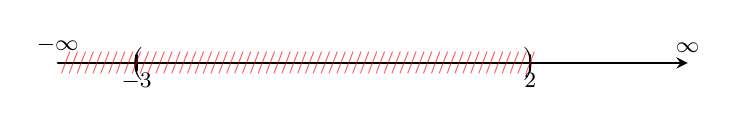
\begin{tikzpicture}[thick, font=\footnotesize, line cap=round,line join=round, >=stealth]
				\draw[-stealth] (-4,0)node[above]{$-\infty$}--(-3,0)node[below]{$-3$}--(2,0)node[below]{$2$}--(4,0)node[above]{$\infty$};
				\draw (-3,.1)--(-3,-.1) (2,.1)--(2,-.1);
				\node at (-3,0) {$\big($};
				\node at (2,0) {$\big)$};
				\foreach \x in {-3.9,-3.8,...,2}{
					\draw[red,opacity=.7] (\x,0)node{$ / $};
					}
			\end{tikzpicture}
		\end{center}
		Vậy $B\setminus A = [2;+\infty)$.
	}
\end{ex}
%Câu34
\begin{ex}%[0H1B2-2]%[Dự án đề kiểm tra HKI NH22-23- Phan Trung Hiếu]%[THPT Chuyên Quốc học - Huế]
	Cho hình bình hành $ABCD$ có $AB=7$, $BC=10$ và $\widehat{ABC}=30^\circ$. Tính diện tích $S$ của hình bình hành $ABCD$.
	\choice
	{$S=\dfrac{35}{2}$}
	{\True$S=35$}
	{$S=70$}
	{$S=\dfrac{35\sqrt{3}}{2}$}
	\loigiai{
		\begin{center}
			\begin{tikzpicture}[font=\footnotesize,thick]
				\path 
				(0,0) coordinate (B)
				(4,0) coordinate (C)
				(1,2) coordinate (A)
				($(A)+(C)-(B)$) coordinate (D)
				;
				\draw (A)--(B)--(C)--(D)--cycle (A)--(C);
				\foreach \x/\g in {C/0,D/30,A/90,B/180}
				\fill[black] 	(\x) circle (1pt)
				($(\g:3mm)+(\x)$) node {$\x$};
			\end{tikzpicture}
		\end{center}
		Ta có $S_{ABC}=\dfrac{1}{2}AB\cdot BC\cdot\sin\widehat{ABC}=\dfrac{1}{2}\cdot7\cdot10\cdot\sin30^\circ=\dfrac{35}{2}$.\\Do đó, $S_{ABCD}=2S_{ABC}=2\cdot\dfrac{35}{2}=35$.
	}
\end{ex}
%Câu35
\begin{ex}%[0H2B2-4]%[Dự án đề kiểm tra HKI NH22-23- Phan Trung Hiếu]%[THPT Chuyên Quốc học - Huế]
	Cho hình bình hành $ABCD$, tâm $O$. Điểm $M$ nào sau đây thõa mãn đẳng thức $\vv{MB}+\vv{MD}=\vv{AB}$?
	\choice
	{$M$ là trung điểm của $AB$}
	{$M$ là trung điểm của $BC$}
	{$M$ là trung điểm của $AO$}
	{\True $M$ là trung điểm của $AD$}
	\loigiai{
			\begin{center}
			\begin{tikzpicture}[font=\footnotesize,thick]
				\path 
				(0,0) coordinate (A)
				(4,0) coordinate (D)
				(1,2) coordinate (B)
				($(D)+(B)-(A)$) coordinate (C)
				($(A)!.5!(D)$) coordinate (M)
				($(B)!.5!(D)$) coordinate (O)
				;
				\draw (A)--(B)--(C)--(D)--cycle (B)--(D) (A)--(C);
				\foreach \x/\g in {A/180,D/0,C/30,B/180,M/-90,O/90}
				\fill[black] 	(\x) circle (1pt)
				($(\g:3mm)+(\x)$) node {$\x$};
			\end{tikzpicture}
		\end{center}
		Ta có
		\begin{equation*}
			\vv{MB}+\vv{MD}=\vv{AB}\Leftrightarrow\vv{MA} +\vv{AB} +\vv{MD}=\vv{AB}\Leftrightarrow\vv{MA}+\vv{MD}=\vv{0}. 
		\end{equation*}
		Vậy $M$ là trung điểm của $AD$.
	}
\end{ex}


\Closesolutionfile{ans}
%\begin{center}
%	\textbf{ĐÁP ÁN}
%	\inputansbox{10}{ans/ans}	
%\end{center}
\begin{center}
	\textbf{PHẦN 2 - TỰ LUẬN}
\end{center}


%Bài 1
\begin{bt}%[0H3B2-3]%[0H3B1-3]%[0H3G1-3]%[Dự án đề kiểm tra HKII NH22-23- Mui Doan]%[THPT chuyên Quốc học Huế]
	Trong mặt phẳng tọa độ $Oxy$, cho $A(3;0)$, $B(4;5)$ và $C(-2;1)$.
	\begin{enumerate}
		\item Chứng minh rằng $A$, $B$, $C$ là $3$ đỉnh của một tam giác cân.
		\item Gọi $G$ là trọng tâm tam giác $ABC$. Tìm tọa độ điểm $D$ là điểm đối xứng với $B$ qua $G$.
		\item Tìm tọa độ điểm $M$ trên đường thẳng $BC$ sao cho $\overrightarrow{AM}\cdot \overrightarrow{BC}= -52$.
	\end{enumerate}
\loigiai{
	\begin{enumerate}
		\item Ta có $\overrightarrow{AB}=(1;5)$; $\overrightarrow{AC}=(-5;1)$.\\
		Vì $1\cdot 1-(-5)\cdot (-5)=-24\neq 0 $ nên $\overrightarrow{AB}$; $\overrightarrow{AC}$ cùng phương. Suy ra $A$, $B$, $C$ không thẳng hàng.\\
		Mà $AB=AC=\sqrt{1^2+5^2}=\sqrt{(-5)^2+1^2}=\sqrt{26}$ nên $A$, $B$, $C$ là $3$ đỉnh của một tam giác cân.
		\item 
		\immini{
		Vì $G$ là trọng tâm tam giác $ABC$ nên $\heva{&x_G=\dfrac{x_A+x_B+x_C}{3}=\dfrac{3+4+(-2)}{3}=\dfrac{5}{3}\\&y_G=\dfrac{y_A+y_B+y_C}{3}=\dfrac{0+5+1}{3}=2.}$\\
		Vì $D$ là điểm đối xứng với $B$ qua $G$ nên $B$ là trung điểm của $DG$.\\
		Ta có
		\allowdisplaybreaks
		\begin{align*}
			&\heva{&x_G=\dfrac{x_D+x_B}{2}\\&y_G=\dfrac{y_D+y_B}{2}}
			\\
			\Leftrightarrow&\heva{&x_D=2x_G-x_B=\dfrac{10}{3}-4=-\dfrac{2}{3}\\&y_D=2y_G-y_B=4-5=-1.}
		\end{align*}
		}
		{
		\begin{tikzpicture}[declare function={r=3;}]
			%Tọa độ đỉnh và góc ở đáy
			\tikzset{declare function={gocA=90;gocB=55;}}
			\path (gocA:r) coordinate (A)
			({gocA+2*gocB}:r) coordinate (B)
			({gocA-2*gocB}:r) coordinate (C)
			($(B)!.5!(C)$) coordinate (N)
			($(A)!2/3!(N)$) coordinate (G)
			($(G)!-1!(B)$) coordinate (D)
			;
			\path (A)--(B) node[midway,sloped]{\tikz{\draw (-90:1pt)--(90:1pt);}};
			\path (A)--(C) node[midway,sloped]{\tikz{\draw (-90:1pt)--(90:1pt);}};
			\draw (A)--(B)--(C)--cycle (A)--(N) (B)--(D);
			\foreach \t/\g in {A/90,B/160,C/0,N/-90,G/-60,D/60}{
				\draw[fill=black] (\t) circle (1pt) node[shift={(\g:7pt)},font=\scriptsize]{$ \t $};
			}
		\end{tikzpicture}
		}
		Vậy $D\left(-\dfrac{2}{3};-1\right)$.
		\item Đặt $M(a;b)$.\\
		Ta có $\overrightarrow{AM}=(a-3;b)$, $\overrightarrow{BC}=(-6;-4)$.\\
		\allowdisplaybreaks
		\begin{align*}
			&\overrightarrow{AM}\cdot \overrightarrow{BC}= -52
			\\
			\Leftrightarrow\,\,&-6(a-b)-4b=-52
			\\
			\Leftrightarrow\,\,&-6a+2b=-52. \qquad(1)
		\end{align*}
		Vì $M\in BC$ nên $\overrightarrow{BM}=(a-4;b-5)$ cùng phương $\overrightarrow{BC}$.\\
		Do đó ta có $\dfrac{a-4}{-6}=\dfrac{b-5}{-4}\Leftrightarrow -4a+16=-6b+30\Leftrightarrow -4a+6b=14$. $\qquad(2)$\\
		Từ $(1)$ và $(2)$ suy ra $\heva{&a=\dfrac{85}{7}\\&b=\dfrac{73}{7}.}$\\
		Vậy $M\left(\dfrac{85}{7};\dfrac{73}{7}\right)$.
	\end{enumerate}
	}
\end{bt}
%Bài 2
\begin{bt}%[0H1B2-1]%[0H1B2-3]%[0H2G3-8]%[Dự án đề kiểm tra HKII NH22-23- Mui Doan]%[THPT chuyên Quốc học Huế]
	Cho tam giác $ABC$ có $AB = a$, $AC = a\sqrt{3}$, $\widehat{BAC} = 30^\circ$.
	\begin{enumerate}
		\item Tính độ dài cạnh $BC$ và bán kính đường tròn ngoại tiếp tam giác $ABC$.
		\item Gọi $M$ là điểm thỏa mãn hệ thức $\overrightarrow{BM}=2 \overrightarrow{MC}$. Chứng minh rằng $\overrightarrow{AM}=\dfrac{1}{3}\overrightarrow{AB}+\dfrac{2}{3}\overrightarrow{AC}$ .
		\item Cho $I$ là một điểm thuộc cạnh $AC$. Tìm giá trị nhỏ nhất của biểu thức $$P=\left| 4\overrightarrow{IA}+\overrightarrow{IB}+\overrightarrow{IC}\right|+6\left|\overrightarrow{IA}-\overrightarrow{IB}+\overrightarrow{IC}\right|.$$
	\end{enumerate}
	\loigiai{
		\begin{center}
			\begin{tikzpicture}
			\path (0,0) coordinate (B)++
			(1,4) coordinate (A)
			($(A)!1!30:(B)$)  coordinate (x)
			(intersection of B--(1,0) and A--x)  coordinate (C)
			($(B)!2/3!(C)$) coordinate (M)
			($(B)!.5!(C)$) coordinate (P)
			($(A)!2/3!(P)$) coordinate (G)
			($(A)!.5!(G)$) coordinate (K)
			;
			\draw (A)--(B)--(C)--cycle (A)--(P) (A)--(M);
			\foreach \t/\g in {A/90,B/180,C/0,M/-90,P/-90,G/180,K/200}{
				\draw[fill=black] (\t) circle (1pt) node[shift={(\g:7pt)},font=\scriptsize]{$ \t $};
			}
			\end{tikzpicture}
		\end{center}
		\begin{enumerate}
			\item Theo định lí co-sin ta có 
			\allowdisplaybreaks
			\begin{align*}
				BC^2&=AB^2+AC^2-2\cdot AB\cdot AC\cdot \cos \widehat{BAC}
				\\
				&=a^2+3a^2-a\cdot a\sqrt{3}\cdot \cos 30^\circ
				\\
				&=\dfrac{5a^2}{2}.
			\end{align*}
			Suy ra $BC=\dfrac{a\sqrt{10}}{2}$.\\
			Theo định lí sin ta có $R=\dfrac{BC}{2\sin \widehat{BAC}}=\dfrac{\dfrac{a\sqrt{10}}{2}}{2\cdot\dfrac{1}{2}}=\dfrac{a\sqrt{10}}{2} $.
			\item Ta có
			\allowdisplaybreaks
			\begin{align*}
				&\overrightarrow{BM}=2 \overrightarrow{MC}
				\\
				\Leftrightarrow\,\,&\overrightarrow{BA}+\overrightarrow{AM}=2\left( \overrightarrow{MA}+\overrightarrow{AC}\right)
				\\
				\Leftrightarrow\,\,&-\overrightarrow{AB}+\overrightarrow{AM}=2\left(- \overrightarrow{AM}+\overrightarrow{AC}\right)
				\\
				\Leftrightarrow\,\,&3\overrightarrow{AM}= \overrightarrow{AB}+2\overrightarrow{AC}
				\\
				\Leftrightarrow\,\,&\overrightarrow{AM}=\dfrac{1}{3} \overrightarrow{AB}+\dfrac{2}{3} \overrightarrow{AC}.
			\end{align*}
			\item Gọi $G$ là trong tâm $\triangle ABC$. Ta có $\overrightarrow{GA}+\overrightarrow{GB}+\overrightarrow{GC}=\overrightarrow{0}$.
			\\
			Ta có 
			\allowdisplaybreaks
			\begin{align*}
				P&=\left| 4\overrightarrow{IA}+\overrightarrow{IB}+\overrightarrow{IC}\right|+6\left|\overrightarrow{IA}-\overrightarrow{IB}+\overrightarrow{IC}\right|
				\\
				&=\left| 6\overrightarrow{IM}+4\overrightarrow{MA}+\overrightarrow{MB}+\overrightarrow{MC}\right|+6\left|\overrightarrow{IM}+\overrightarrow{MA}-\overrightarrow{MB}+\overrightarrow{MC}\right|
				\\
				&=\left| 6\overrightarrow{IM}+4\left(-\dfrac{1}{3} \overrightarrow{AB}-\dfrac{2}{3} \overrightarrow{AC}\right)-\dfrac{2}{3}\overrightarrow{BC}+\dfrac{1}{3}\overrightarrow{BC}\right|+6\left|\overrightarrow{IM}-\dfrac{1}{3} \overrightarrow{AB}-\dfrac{2}{3} \overrightarrow{AC}+\overrightarrow{BC}\right|
				\\
				&=\left| 6\overrightarrow{IM}-\dfrac{4}{3} \overrightarrow{AB}-\dfrac{8}{3} \overrightarrow{AC}-\dfrac{2}{3}\left(\overrightarrow{AC}-\overrightarrow{AB}\right)+\dfrac{1}{3}\left(\overrightarrow{AC}-\overrightarrow{AB}\right)\right|+6\left|\overrightarrow{IM}-\dfrac{1}{3} \overrightarrow{AB}-\dfrac{2}{3} \overrightarrow{AC}+\overrightarrow{AC}-\overrightarrow{AB}\right|
				\\
				&=\left| 6\overrightarrow{IM}-\overrightarrow{AB}-3\overrightarrow{AC}\right|+\left|6\overrightarrow{IM}-8\overrightarrow{AB}+2\overrightarrow{AC}\right|
				\\
				&=\left| 6\overrightarrow{IM}-\overrightarrow{AB}-3\overrightarrow{AC}\right|+\left|-6\overrightarrow{IM}+8\overrightarrow{AB}-2\overrightarrow{AC}\right|
				\\
				&\geq \left| 6\overrightarrow{IM}-\overrightarrow{AB}-3\overrightarrow{AC}-6\overrightarrow{IM}+8\overrightarrow{AB}-2\overrightarrow{AC}\right|
				\\
				&=\left| 7\overrightarrow{AB}-5\overrightarrow{AC}\right|\geq \left| \left|7\overrightarrow{AB}\right|-\left|5\overrightarrow{AC}\right|\right|
				\\
				&=\left|7a-5a\sqrt{3}\right|=5a\sqrt{3}-7a.
			\end{align*}
		Vậy $\min P=5a\sqrt{3}-7a$.
		\end{enumerate}
	}
\end{bt}
